
\chapter{Chapter 4. Methodology}
\label{ch:methodology}

\section{Experimental Design}
\label{sec:exp_design}

The goal of this thesis is to compare embedding compression methods in
identical conditions. Prior work makes this hard. As shown in
Section~\ref{sec:related}, each study has a different background, training
data, and benchmarks. This thesis controls all three.

All methods studied here are applied to the same set of backbone models. They
are fine-tuned under the same conditions and are evaluated on the same
benchmark. Figure~\ref{fig:methodology_overview} shows that the experiments
are set up into two tracks. Both begin with the same pre-trained weights.

\begin{figure}[!h]
  \centering
  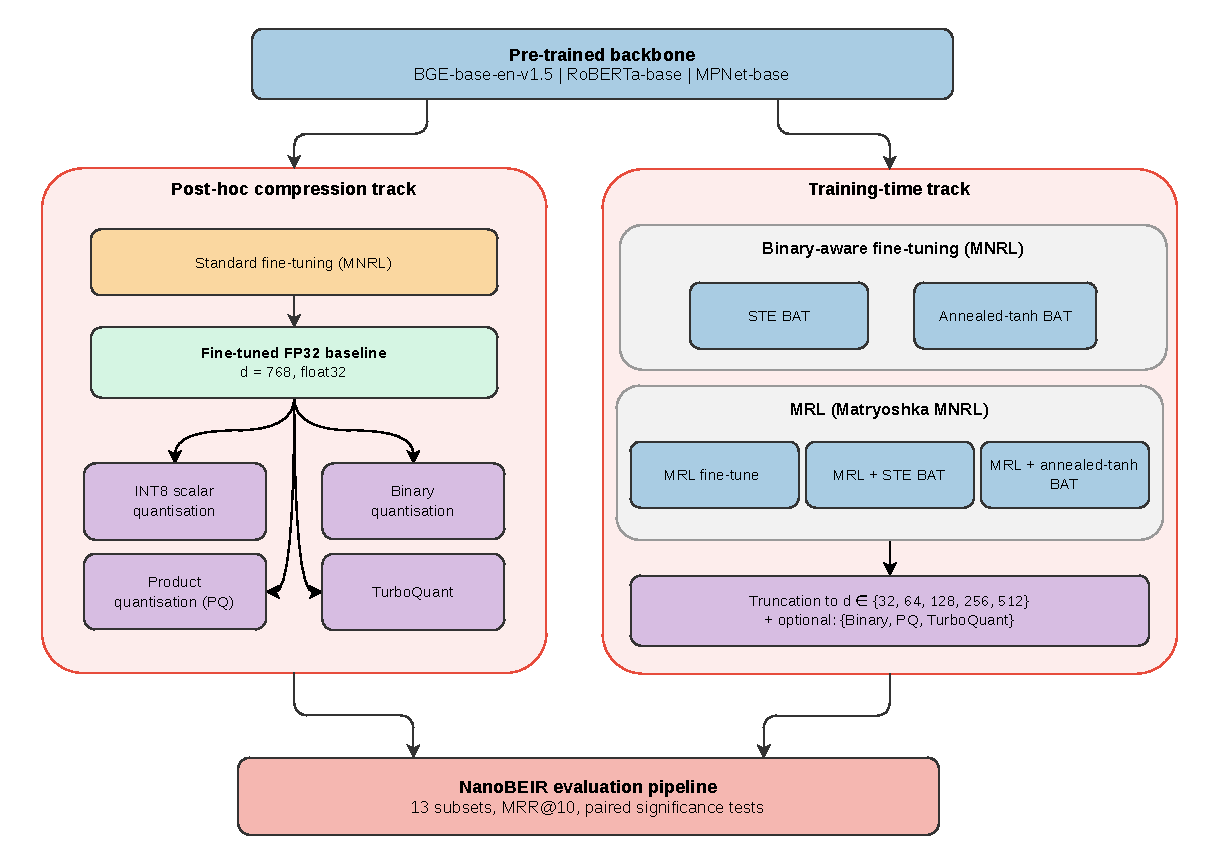
\includegraphics[width=\textwidth]{Figures/methodology_main.pdf}
  \caption[Overview of the experimental methodology.]{%
  Overview of the experimental methodology. There are two separate tracks
  for each pre-trained backbone (BGE-base-en-v1.5, RoBERTa-base, and
  MPNet-base). The post-hoc compression track fine-tunes a fp32 baseline
  and then compresses the cached embeddings with INT8, binary, PQ, or
  TurboQuant. The training-time track changes the architecture or loss:
  STE or annealed-tanh binarization-aware training (BAT), Matryoshka
  Representation Learning (MRL), and versions that use both MRL and BAT.
  Checkpoints in MRL also allow post-hoc truncation to
  $d \in \{32, 64, 128, 256, 512\}$, which can be stacked with binary, PQ,
  or TurboQuant. All resulting variants are evaluated on the NanoBEIR
  benchmark with paired significance tests.}
  \label{fig:methodology_overview}
\end{figure}

\paragraph{Post-hoc track.} Each backbone is fine-tuned without any
compression. After that, various post-hoc compression methods are applied to
the embeddings. The compression step does not affect the checkpoint itself.

\paragraph{Training-time track.} Each backbone is fine-tuned with a modified
architecture, a modified loss, or both. The fine-tuned fp32 baseline is not
where this track starts. Like the post-hoc track, it starts with backbone
weights that have already been trained.

All variants are evaluated on NanoBEIR using the pipeline described in
Section~\ref{sec:eval_framework}. Table~\ref{tab:experiment_summary} lists the
six training variants and the post-hoc transforms applied to each.

\begin{table}[H]
  \centering
  \caption[Summary of training variants and applicable post-hoc transforms.]{Summary of training variants. Each variant is a complete fine-tuning run from a pre-trained backbone. Post-hoc transforms are applied after training with no weight modification.}
  \label{tab:experiment_summary}
  \resizebox{\columnwidth}{!}{%
  \begin{tabular}{| l | l | l | l |}
    \hline
    \textbf{Variant} & \textbf{Architecture change} & \textbf{Loss function} & \textbf{Post-hoc options} \\ [0.5ex] \hline
    Fine-tuned fp32 baseline         & None                         & MNRL                  & INT8, Binary, PQ, TurboQuant         \\ \hline
    STE binarization-aware           & $+$ BinarizationLayer (STE)  & MNRL                  & Binary                               \\ \hline
    MRL                              & None                         & MatryoshkaLoss (MNRL) & Truncation; Truncation $+$ INT8/Binary \\ \hline
    MRL $+$ STE                      & $+$ BinarizationLayer (STE)  & MatryoshkaLoss (MNRL) & Truncation; Truncation $+$ Binary    \\ \hline
    Annealed tanh binarization-aware & $+$ AnnealedTanhLayer        & MNRL                  & Binary                               \\ \hline
    MRL $+$ Annealed tanh            & $+$ AnnealedTanhLayer        & MatryoshkaLoss (MNRL) & Truncation; Truncation $+$ Binary    \\ \hline
  \end{tabular}}
\end{table}


\section{Training Setup}
\label{sec:training_infra}

All training variants are run independently on three backbone architectures:
BGE-base-en-v1.5, RoBERTa-base, and MPNet-base
(Section~\ref{sec:biencoder}).

The training objective is the Multiple Negatives Ranking Loss (MNRL,
Section~\ref{sec:contrastive}) computed with cosine similarity and with
in-batch negatives. Batches are sampled from the seven-dataset training
mixture (Chapter~3).

The fine-tuned fp32 baseline is trained by this setup with no compression
layer. It acts as the starting point for all post-hoc compression methods.
Training-time variants use the same training setup but modify the
architecture, the loss, or both (Section~\ref{sec:training_time}). They
fine-tune from the pre-trained backbone weights, not from the baseline
checkpoint. All variants and backbones use the same hyperparameters. The
arrangement is summed up in Table~\ref{tab:hyperparams}.

\begin{table}[H]
  \centering
  \caption[Training hyperparameters.]{Training hyperparameters shared across all experiments and backbone models. Effective batch size accounts for per-device batch, number of GPUs, and gradient accumulation.}
  \label{tab:hyperparams}
  \begin{tabular}{| l | l |}
    \hline
    \textbf{Hyperparameter}     & \textbf{Value} \\ [0.5ex] \hline
    Optimizer                   & AdamW \\ \hline
    Learning rate               & $2\times10^{-5}$ \\ \hline
    LR scheduler                & Linear decay with warmup \\ \hline
    Warmup ratio                & 0.10 \\ \hline
    Weight decay                & 0.10 \\ \hline
    Per-device batch size       & 16 \\ \hline
    Gradient accumulation steps & 8 \\ \hline
    Effective batch size        & 512 \quad ($16 \times 4\ \text{GPUs} \times 8\ \text{steps}$) \\ \hline
    Training epochs             & 1 \\ \hline
    Max sequence length         & 512 tokens \\ \hline
    Precision                   & bfloat16 \\ \hline
  \end{tabular}
\end{table}


\section{Training-Time Compression Experiments}
\label{sec:training_time}

Each variant below modifies the architecture, the loss, or both. All other
settings follow Section~\ref{sec:training_infra}.

\subsection{STE Binarization-Aware Training}
\label{sec:bat_ste}

The STE binarization layer (Section~\ref{sec:compression_bg}) is added
after mean pooling, and MNRL is computed on the binarized outputs.

\subsection{MRL Fine-Tuning}
\label{sec:mrl_train}

The architecture is identical to the baseline; only the loss changes. The
Matryoshka loss (Section~\ref{sec:compression_bg}, Equation~\ref{eq:mrl})
wraps MNRL, with all six losses weighted equally ($c_m = 1$). The
full-dimension loss ($d = 768$) is retained to prevent degradation of the
complete representation. Truncation to $d' \in \{32, 64, 128, 256, 512\}$
is applied post-hoc by the evaluation pipeline (Section~\ref{sec:stacked_method}).

\subsection{Joint MRL and STE Binarization-Aware Training}
\label{sec:mrl_bat}

This variant applies both the binarization layer of Section~\ref{sec:bat_ste}
and the Matryoshka loss of Section~\ref{sec:mrl_train}.

\subsection{Annealed Tanh Binarization-Aware Training}
\label{sec:bat_atanh}

The STE binarization layer of Section~\ref{sec:bat_ste} is replaced with
the annealed-tanh surrogate (Section~\ref{sec:compression_bg}). The
annealing rate is $\gamma = 0.1$, following~\cite{yamada2021efficient};
empirical validation across $\gamma \in \{0.05, 0.1, 0.2\}$ is reported
in Table~\ref{tab:gamma_ablation}. Over the $\sim$8{,}000 global steps
of one epoch, $\beta$ grows from 1 to approximately 28. MNRL is computed
on the soft-binarized embeddings.

\subsection{Joint MRL and Annealed Tanh Binarization-Aware Training}
\label{sec:mrl_atanh}

This variant combines the annealed-tanh layer of Section~\ref{sec:bat_atanh}
with the Matryoshka loss of Section~\ref{sec:mrl_train}.


\section{Post-Hoc Compression}
\label{sec:posthoc}

Post-hoc methods are applied to the cached embeddings of the fine-tuned fp32
baseline.

\subsection{INT8 Scalar Quantization}

The first 1{,}000 corpus embeddings are used to calibrate the quantizer
(Section~\ref{sec:compression_bg}, Equation~\ref{eq:int8}) by finding the
range of embedding values. At retrieval time the int8 values are scored
directly with cosine similarity. Since cosine is scale-invariant, this
yields the same ranking as scoring the dequantized vectors.

\subsection{Binary Quantization}

Bits are packed into \texttt{uint8}, and similarity is Hamming distance
between the binary query and corpus vectors
(Section~\ref{sec:compression_bg}).

\subsection{Product Quantization}

PQ is fitted on the corpus embeddings using Faiss~\cite{douze2024faiss}.
Sub-vector counts $M \in \{16, 24, 32, 48, 64, 96, 128, 192\}$ are evaluated
with centroid bit-widths $n_{\text{bits}} \in \{4, 8\}$.

\subsection{TurboQuant}

TurboQuant~\cite{zandieh2025turboquant} is calibrated on the corpus
embeddings. Bit-depths of $\{1, 2, 3, 4, 8\}$ bits per dimension are evaluated.


\section{Stacked Combinations}
\label{sec:stacked_method}

MRL-trained checkpoints support simultaneous compression along two
dimensions: dimensionality reduction via post-hoc truncation, followed by a
precision-reducing transform. After each MRL checkpoint is truncated to
each of the five granularities $\{32, 64, 128, 256, 512\}$, binary
quantization, PQ, or TurboQuant is applied to the truncated embedding. This
yields the grid of (backbone $\times$ truncation dimension $\times$
precision method) combinations evaluated in Chapter~5.


\section{Evaluation Framework}
\label{sec:eval_framework}

\subsection{Embedding Cache and Transform Pipeline}

Each checkpoint encodes the NanoBEIR corpus and the queries into float32
embeddings that are cached. All compression variants are applied on the
cached embeddings. A compression variant applies dimensionality reduction
with at most one precision-reducing transform listed below.
%
\begin{enumerate}
  \item Binary quantization with \texttt{uint8} packing.
  \item INT8 scalar quantization.
  \item Product quantization (PQ).
  \item TurboQuant.
\end{enumerate}

\subsection{Metrics}
\label{sec:metrics}

The three retrieval metrics used in this thesis, NDCG@$k$, MRR@$k$, and
Recall@$k$, are defined in Section~\ref{sec:ir_eval}. All are computed at
$k \in \{1, 3, 5, 10\}$, averaged over the 50 queries per NanoBEIR subset,
then macro-averaged across the 13 subsets. MRR is the primary reported
metric throughout Chapter~5.

\subsection{Memory Budget and Compression Ratio}
\label{sec:memory}

Embedding memory is computed as:
%
\begin{equation}
  \text{memory (bytes)} = n \times d_{\text{stored}} \times \frac{b}{8},
  \label{eq:memory}
\end{equation}
%
where $n$ is the number of embeddings, $d_{\text{stored}}$ is the stored
dimension (number of PQ sub-spaces for PQ variants), and $b$ is the number
of bits per stored element. For float32, $b = 32$; for INT8, $b = 8$; for
binary packed embeddings, $b = 1$.

The compression ratio $r$ is computed by dividing the original embedding
size by the new size. A float32 vector of 768 dimensions takes 3{,}072
bytes. For each method family, the ratio looks like this:
%
\begin{itemize}
  \item Scalar precision reduction to $b$ bits per component:
        $r = 32 / b$ (INT8: $4\times$; binary: $32\times$).
  \item MRL truncation to $d'$ dimensions: $r = 768 / d'$.
  \item Product quantization with $M$ sub-spaces and $n$-bit codes per
        sub-space: $r = (768 \times 32) / (M \times n)$.
  \item TurboQuant at $b$ bits per dimension: $r = 32 / b$.
\end{itemize}
%
Stacked combinations multiply the per-axis ratios. For example,
MRL-256 followed by binary quantization gives
$(768/256) \times 32 = 96\times$ compression.

\subsection{Statistical Significance Testing}
\label{sec:significance}

The tests used here are defined in Section~\ref{sec:significance_bg}. For each
model pair, per-query scores are collected across all 13 NanoBEIR subsets
and pooled into a single paired sample (649 query pairs per comparison). The
per-query difference is $d_i = s_A(q_i) - s_B(q_i)$ for each query $q_i$,
where $s(\cdot)$ denotes the retrieval score of the respective model. The Shapiro--Wilk test is first applied to this vector of differences to
assess normality. If normality is not rejected, the paired $t$-test is used;
otherwise the Wilcoxon signed-rank test is used. Cohen's $d$ is reported as
an effect size in either case. Results in Chapter~5 are flagged as
statistically significant at $\alpha = 0.05$.
